\section{Comparative Analysis}\label{comparativeAnalysis}

Conducting a comparative analysis of 3D models presents a challenging endeavor, as the parameters defining their success vary widely based on the intended application. For instance, low-resolution models suffice for real-time rendering in virtual reality or gaming contexts, whereas the film industry demands high-quality renderings. Similarly, in industrial applications, precision down to the millimeter is crucial, necessitating extremely detailed and accurate meshes.

In light of these diverse requirements, this analysis of Section~\ref{comparativeAnalysis} evaluates the generated models across multiple dimensions:

\begin{enumerate}
    \item \textbf{Prompt/Result Fidelity:} Investigates how closely each model aligns with the provided prompt or image. Can the intended subject be identified without prior knowledge of the input?
    \item \textbf{Detail Level:} Examines the intricacy of each model. Are the models finely detailed or do they exhibit a more generalized structure?
    \item \textbf{Texture Realism:} Assesses the authenticity and quality of the model textures. How `real' do they look like?
    \item \textbf{Topology:} Looks into the smoothness or blockiness of the model's surface. Is the topology uniformly smooth or does it exhibit a more fragmented appearance?
    \item \textbf{Model Integrity:} Considers whether the model is a single, cohesive unit or split into multiple segments.
\end{enumerate}

Additionally, technical aspects of each model are analyzed, such as the time required for rendering, efficiency, and resource consumption. Each method is also subjected to specific tests based on particular requirements. For example, when symmetry is a key factor, models are evaluated on their ability to produce symmetric outputs. Similarly, when smoothness is crucial, special attention is given to the topology.

The technical metrics for this analysis are derived from the tensorboard and outputs generated during the training process. The percentages and detailed assessments of geometrical features like symmetry, topology, and the presence of holes in the models are calculated using Evaluate3D. This tool, developed as part of this research, leverages the trimesh Python library \citep{trimesh} to extract detailed insights into the fundamental geometric properties of each 3D model.

In the preceding section, it was observed that the methods yielded diverse outcomes when tasked with a broad prompt, such as creating a `robot made of plants'. The text-to-3D methods faced challenges in initially generating an object, a stark contrast to the image-to-3D methods that benefited from having a reference image, offering some directional guidance and hence a slight advantage. To establish a more leveled playing field for the various methods, the next prompt chosen for testing was ``a high-quality rendering of a Playmobil firefighter''. Playmobil figures are known for their uniform base structures, differing primarily in clothing or texture. This prompt was therefore selected to assess whether a method could accurately capture the fundamental structure dictated by the prompt. The outcomes of each method, applied to this specific prompt, are illustrated in Figure~\ref{fig:resultPlaymobil}.

% Magic123
\begin{figure}[ht]
    \centering
    \begin{subfigure}[b]{0.222\textwidth}
        \centering
        \fontsize{9pt}{7pt}\selectfont\text{Iteration = 100}\vspace{.1cm}
        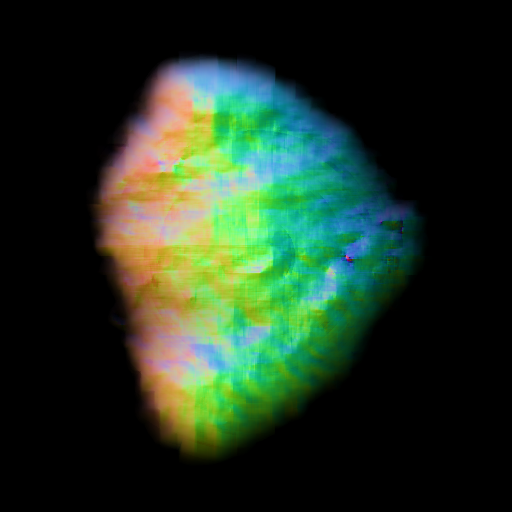
\includegraphics[width=\textwidth]{etc/a robot made out of plants/magic123/magic123_coarse_robot_right_0_part2.png}
        \caption{}
    \end{subfigure}
    \begin{subfigure}[b]{0.222\textwidth}
        \centering
        \fontsize{9pt}{7pt}\selectfont\text{It. 5000}\vspace{.1cm}
        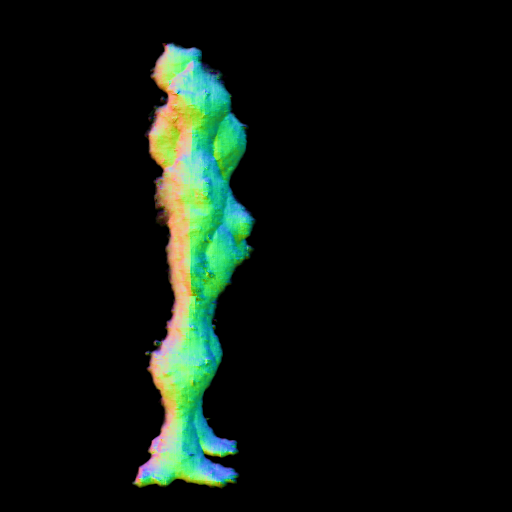
\includegraphics[width=\textwidth]{etc/a robot made out of plants/magic123/magic123_coarse_robot_right_5000_part2.png}
        \caption{}
    \end{subfigure}
    \begin{subfigure}[b]{0.222\textwidth}
        \centering
        \fontsize{9pt}{7pt}\selectfont\text{It. 10000}\vspace{.1cm}
        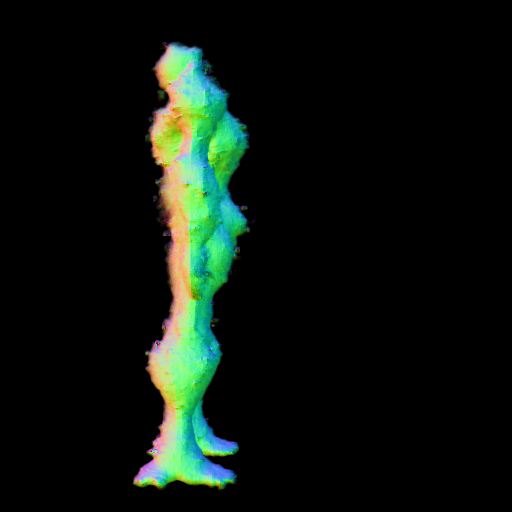
\includegraphics[width=\textwidth]{etc/a robot made out of plants/magic123/magic123_coarse_robot_right_10000_part2.png}
        \caption{}
    \end{subfigure}
    \caption{Results obtained using the prompt ``a high-quality rendering of a Playmobil firefighter''}~\label{fig:resultPlaymobil}
\end{figure}



\begin{table}[h]
    \centering
    \small 
    \begin{tabular}{lcccccccc}
    \toprule
    Prompt & Dreamfusion & \multicolumn{2}{c}{Magic3D} & \multicolumn{2}{c}{Fantasia3D} & \multicolumn{2}{c}{Magic123} & Wonder3D \\
    \cmidrule(r){3-4} \cmidrule(lr){5-6} \cmidrule(l){7-8}
    & & \multicolumn{1}{c}{Coarse} & \multicolumn{1}{c}{Refine} & \multicolumn{1}{c}{Geom.} & \multicolumn{1}{c}{Appear.} & \multicolumn{1}{c}{C.} & \multicolumn{1}{c}{R.} &  \\
    \midrule
    Robot & 1:24 & 1:23 & 1:20 & 1:15 & 1:18 & 1:46 & 1:47 & 0:15 \\
    Playmobil & 1:17 & 1:17 & 1:18 & 1:14 & 1:17 & 1:46 & 1:46 & 0:15 \\
    Fern & 1:25 & 1:24 & 1:19 & 1:17 & 1:20 & 1:52 & 1:48 & 0:15 \\
    Bread & 1:25 & 1:21 & 1:21 & 1:17 & 1:20 & 1:54 & 1:52 & 0:15 \\
    \bottomrule
    \end{tabular}
    \caption{Comparison of Generation Times for Different Prompts Across Methods (Hours:Minutes). Legend: C = Coarse, R = Refine, Geom = Geometry, Appear = Appearance.}~\label{table:generation_times_complex}
\end{table}

    
    
    
    
    
    
    
    
    